\documentclass[tikz]{standalone}

\usetikzlibrary{arrows,calc}

\begin{document}
	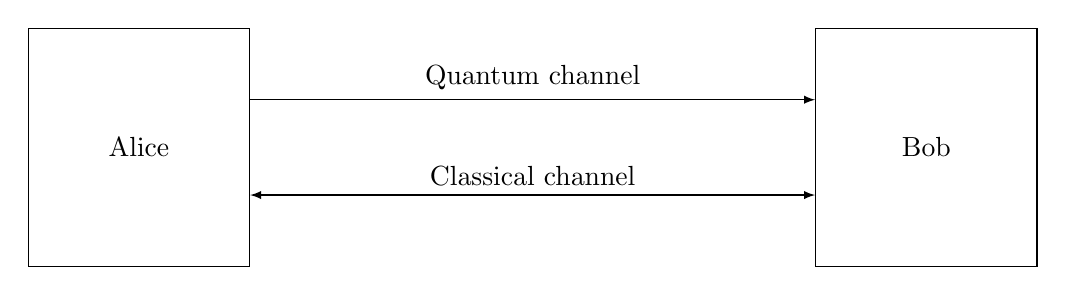
\begin{tikzpicture}[
		node distance=3em,
		arrow/.style={-latex},
		darrow/.style={latex-latex},
		block/.style={draw, minimum height=20ex, minimum width=8em, align=center},
	]
		\node at (0,0) (tx) [block] {Alice};
		\node at (10,0) (rx) [block] {Bob};
		
		\draw[arrow] ([yshift=4ex]tx.east) -- node[anchor=south]{Quantum channel} ([yshift=4ex]rx.west);
		\draw[darrow] ([yshift=-4ex]tx.east) -- node[anchor=south]{Classical channel} ([yshift=-4ex]rx.west);
	\end{tikzpicture}
\end{document}
